\documentclass[xcolor=dvipsnames]{beamer}
%
% Choose how your presentation looks.
%
% For more themes, color themes and font themes, see:
% http://deic.uab.es/~iblanes/beamer_gallery/index_by_theme.html
%

\mode<presentation>

\usetheme{Warsaw}      % or try Darmstadt, Madrid, Warsaw, ...\textbf{\(\(\(\)\)\)}}

\usecolortheme{beaver} % or try albatross, beaver, crane, ...
\usefonttheme{professionalfonts}  % or try serif, structurebold, ...
\setbeamertemplate{navigation symbols}{}
\setbeamertemplate{caption}[numbered]
\usepackage{ragged2e}
\usepackage[spanish]{babel}
\usepackage[utf8x]{inputenc}
\usepackage{graphicx}
\usepackage{lmodern}
\usepackage{multicol}
\usepackage{xcolor}
\usepackage{pgf}
\usepackage{textpos}
\usepackage{tikz}
\usepackage{apacite}
\usepackage{natbib}
\usepackage{stackengine}
\usepackage{amsmath}
\usepackage{algorithm2e}
\usepackage{algorithmic}
\usepackage{caption}
\usepackage{graphicx}
\usepackage{subcaption}
\usepackage{multirow}
\captionsetup[subfigure]{font=scriptsize}
\usepackage{mathtools} % for "\mathclap" macro; loads "amsmath" package
\usepackage{ragged2e}


%\newcommand{\figcite}[3]{
  %\def\stackalignment{l}
  %\stackunder{\includegraphics[width=#1]{#2}}{\scriptsize Source: #3}}

\newcommand\tab[1][1cm]{\hspace*{#1}}

\definecolor{myNewColorText}{RGB}{204,0,0}
%\definecolor{myNewColorBack}{RGB}{79,156,69}
\definecolor{myNewColorBack}{RGB}{91,147,195}
\definecolor{myNewColorTittlePanel}{RGB}{216,216,216}


\newcounter{saveenumi}
\newcommand{\seti}{\setcounter{saveenumi}{\value{enumi}}}
\newcommand{\conti}{\setcounter{enumi}{\value{saveenumi}}}

\resetcounteronoverlays{saveenumi}


\title[MIDAS]{Asociación de variantes en regiones codificantes de genes con datos clínicos en pacientes colombianos usando minería de datos.}
\author[Vélez, Jennifer.]{
    Autor: Jennifer Vélez Segura \\
    Director: Elizabeth León Guzmán \\
    Asesor: Claudia Serrano
}

\institute[U. Nacional de Colombia]
{
	Grupo de Investigación -- MIDAS\\   
    Universidad Nacional de Colombia, Bogot\'{a} D.C., Colombia
}
\date{Mayo 2019}

\setbeamercolor{section in toc}{fg=myNewColorBack}

% Change the background and the color of the text
\setbeamercolor*{palette primary}{bg = myNewColorBack, fg = myNewColorText}
\setbeamercolor*{palette secondary}{fg = myNewColorText}
\setbeamercolor*{palette tertiary}{fg = myNewColorText}
\setbeamercolor*{palette quaternary}{fg = myNewColorText}
\setbeamercolor{titlelike}{parent=structure,bg=myNewColorTittlePanel}


% Setup the bibliography
\setbeamertemplate{bibliography entry title}{}
\setbeamertemplate{bibliography entry location}{}
\setbeamertemplate{bibliography entry note}{}

%\setbeamercolor{block title}{fg=myNewColorText, bg=myNewColorBack}

% Change the color bullets of TOC
\setbeamercolor{section number projected}{bg=myNewColorBack,fg=myNewColorText}
\setbeamercolor{subsection number projected}{bg=myNewColorBack}
\setbeamercolor*{item}{fg=myNewColorBack}

% Change the size of font TOC
%%%%%%%%%%%%%%%%%%%%%%%%%%%%%% User specified LaTeX commands.
%Two column ToC
\setbeamerfont{section in toc}{size= \scriptsize}
\setbeamerfont{subsection in toc}{size= \scriptsize}

% image directory
\graphicspath{ {images/} }

\logo{\pgfputat{\pgfxy(0.3,-0.5)}{\pgfbox[right,base]{
\includegraphics[height=1.2cm ]{midas_logo.png}}}}


\begin{document}

\begin{frame}
  \titlepage
\end{frame}

\begin{frame}{Contenido}
    \begin{columns}[onlytextwidth,T]
        \begin{column}{.55\textwidth}
	            \tableofcontents[sections=1-3]
        \end{column}
        \begin{column}{.60\textwidth}
            \tableofcontents[sections=4-]
        \end{column}
    \end{columns}
\end{frame}

\section{Introducción}

\begin{frame}{Introducción}
    
\justifying
La necesidad de comprender los procesos biológicos que están implicados en las distintas enfermedades, a partir de  la secuenciación del ADN  presentan la oportunidad de aplicar diferentes tipos de análisis que ayuden a entender la relación genotipo-fenotipo. 
\hfill \break 

\begin{figure}
    \centering
    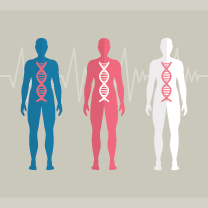
\includegraphics[width=60]{variacionhumna.png}
  \end{figure}
  
\hfill \break
\tiny{https://www.ebi.ac.uk/training/online/course/human-genetic-variation-i-introduction}
\end{frame}

\section{Secuenciación}

\begin{frame}{Análisis de secuencias de ADN}
	
	El proceso de análisis de secuencias se realiza a través de los siguientes pasos:
	
	\begin{itemize}
		\item Extracción de ADN.
		\item Secuenciación de la muestra de ADN.
		\item Obtención de lecturas.
		\item Análisis de genes.
		\item Generación de reportes.
	\end{itemize}
	
\end{frame}

\begin{frame}{Secuenciación}	
	\justifying
	La secuenciación es el proceso químico que permite identificar el orden de nucleótidos en molécula de ADN, ARN o una proteína \cite{Kulski2016}.

	\centering 
	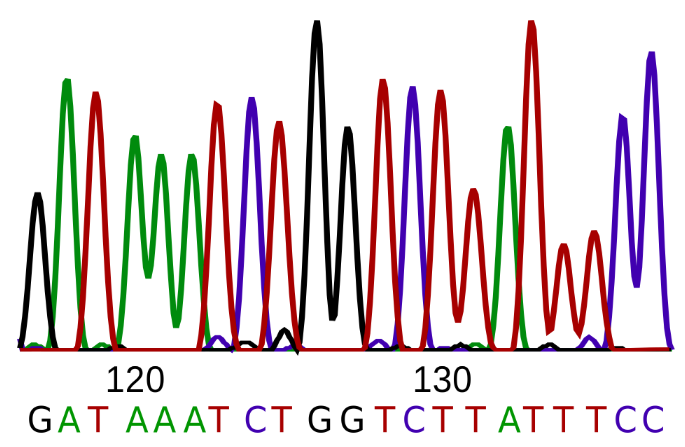
\includegraphics[width=60mm]{secuenciacion}
	
	\hfill \break
	
	\justifying
	\tiny{Tomado de: https://experiment.com/u/v0RZUQ}
\end{frame}

\begin{frame}{Secuenciación de siguiente generación (NGS)}	
	\justifying
	Se han desarrollado diferentes metodologías para realizar secuenciación, estas son conocidas como secuenciación de alto rendimiento y tienen la capacidad de realizar secuenciaciones de manera masiva, rápida y económica  \cite{Kulski2016}. 
	
\hfill \break
	\centering
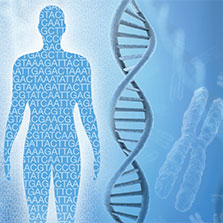
\includegraphics[width=25mm]{ngs.jpg}

\hfill \break

\justifying
\tiny{https://www.almacgroup.com/news/almac-group-to-collaborate-with-illumina-on-next-generation-sequencing-based-companion-diagnostic-development/}
	
\end{frame}

\begin{frame}{Secuenciación con Illumina}
	\centering
	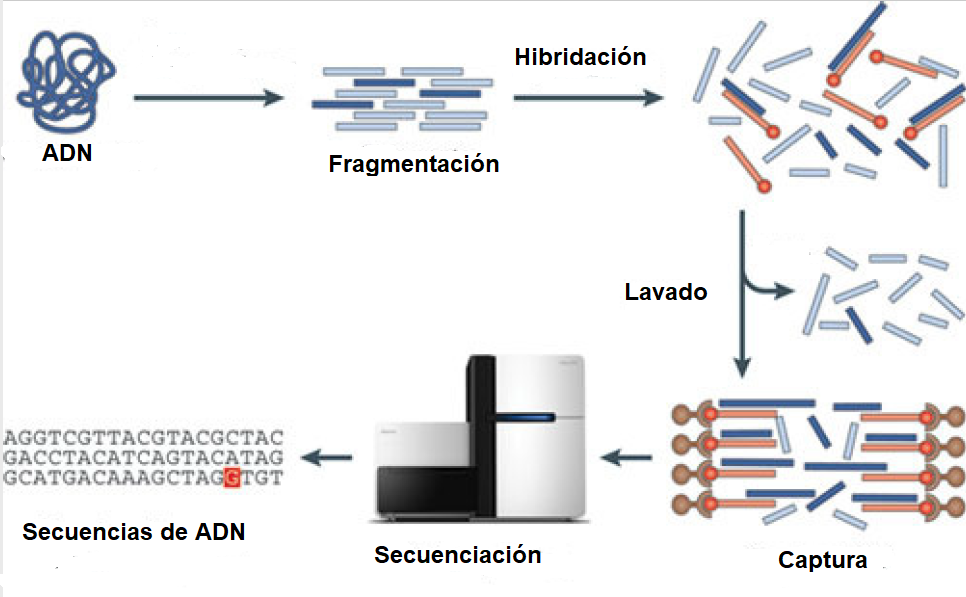
\includegraphics[width=11cm]{secuenciacion1.png}
\end{frame}

\subsection{Alineamiento}

\begin{frame}{Alineamiento}
	\justifying
	Es el proceso de mapear las lecturas secuenciadas usando un genoma de referencia, que para humanos generalmente es el hg19.
	\hfill \break
	
	\begin{figure}
	\centering
	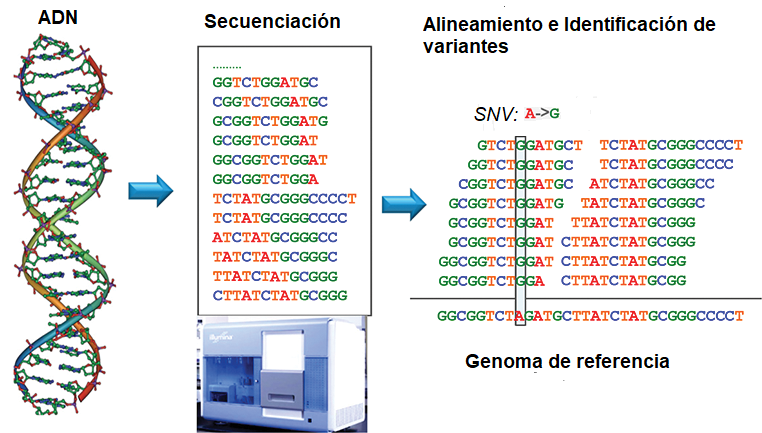
\includegraphics[width=8cm]{resumenngs.png}
	\end{figure}
\justifying
\tiny{https://www.intechopen.com/books/cloud-computing-architecture-and-applications/}	
\end{frame}

\subsection{Variantes}
\begin{frame}{Variantes}
	\begin{figure}
		\centering
		\begin{subfigure}[b]{0.47\textwidth}
			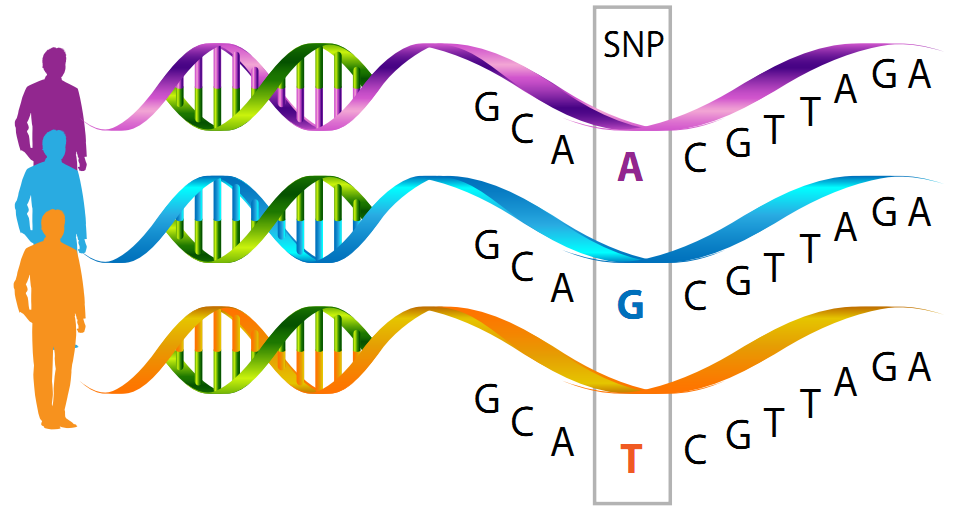
\includegraphics[width=\textwidth]{snp.png}
			\caption{Variante de Nucleótido Simple SNV}
		\end{subfigure}
		~ %add desired spacing between images, e. g. ~, \quad, \qquad, \hfill etc. 
		%(or a blank line to force the subfigure onto a new line)
		\begin{subfigure}[b]{0.47\textwidth}
			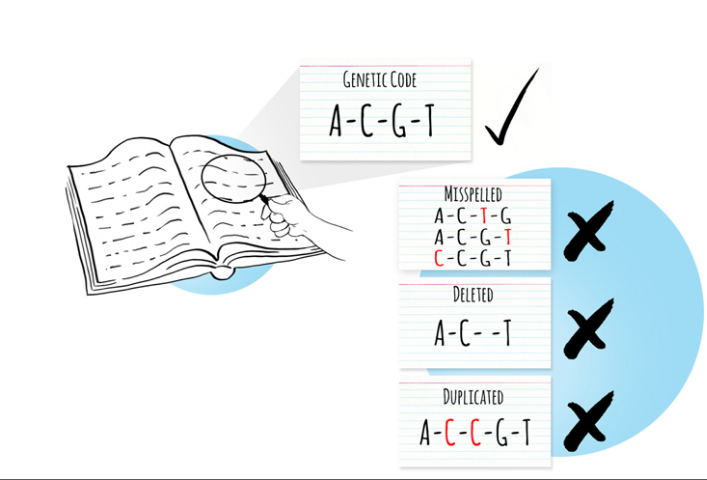
\includegraphics[width=\textwidth]{variante.png}
			\caption{ Variantes Indels}
		\end{subfigure}
		\caption{Tipos de variantes según el cambio de núcleotido}
	\end{figure}
	
\end{frame}

\begin{frame}{Retos para análisis de secuencias}

\begin{enumerate}
	\justifying
	\item No existe un protocolo \textit{``gold standard"} para realizar un análisis de secuencias.
	
	\item Existe una gran cantidad de información obtenida que no es posible de analizar sin utilizar métodos computacionales.
	
	\item La población colombiana no cuenta con estudios de este tipo y no se encuentra caracterizada como otras poblaciones.
	
	\item En la mayoría de los estudios realizados no cuentan con la información clínica.
\end{enumerate}

   
\end{frame}

\subsection{Objetivos}

\begin{frame}{Objetivos}
	
	\begin{block}{}
		{\justifying 
			Proponer un modelo de minería de datos que permita asociar variantes con características clínicas de pacientes colombianos.
		}
	\end{block}
	
	\begin{itemize}
		\item Realizar la identificación de variantes en pacientes colombianos.
		\item Integrar la información clínica con las variantes obtenidas.
		\item Diseñar e implementar un modelo de asociación entre variantes e historias clínicas.
		\item Validar y visualizar los resultados del modelo de minería.
	\end{itemize}
		
\end{frame}

\section{Integración de datos}
\subsection{Datos}

\begin{frame}{Datos}

\begin{block}{Origen de los datos}
	{\justifying 
		Los datos utilizados en el presente trabajo proviene de las historias clínicas de 228 pacientes colombianos, distribuidos en 133 pacientes femeninas y 95 pacientes masculinos secuenciados en regiones codificantes de 4813 genes. 
	}
\end{block}

\textit{Estos datos fueron otorgados por el Laboratorio Genetix S.A.S.}
\end{frame}

\begin{frame}{Modelo propuesto}
\begin{figure}
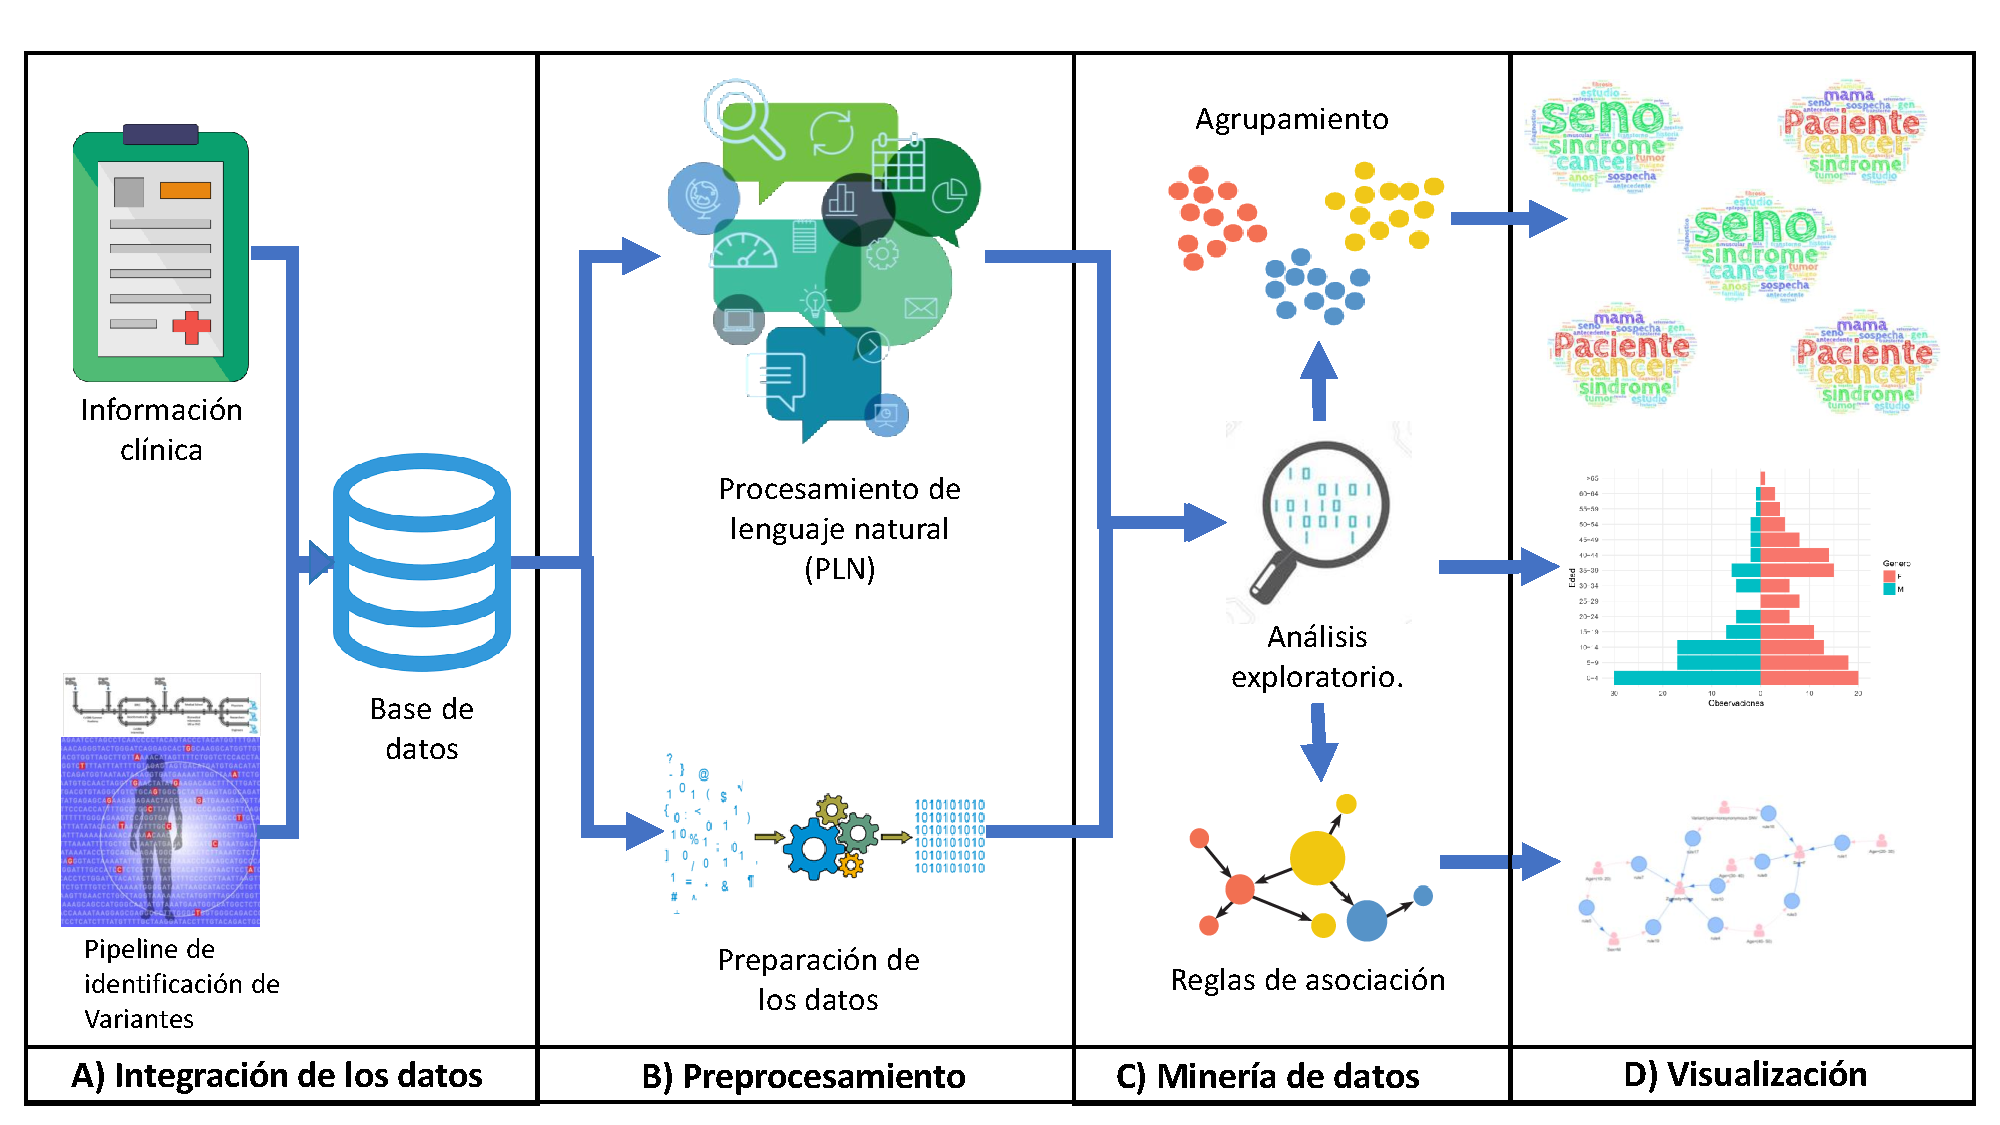
\includegraphics[width=1\textwidth]{KDDtesis.pdf}
\end{figure}
\end{frame}

\begin{frame}{Identificación de variantes}
	\justifying 
	Los pipelines bioinformáticos para NGS son comúnmente desarrollados en una plataforma específica y pueden ser adaptados según las necesidades del laboratorio, la mayoría de los pipelines consisten en los siguientes pasos \cite{Roy2018}:
	\justifying 
	\begin{enumerate}[1.]
		\justifying
		\item Generación de secuencias.
		\item Alineamiento de las secuencias.
		\item Llamado de variantes.
		\item Filtrado de variantes.
		\item Anotación de variantes.
		\item Priorización de variantes. 
	\end{enumerate}
\end{frame}

\begin{frame}{Pipeline implementado en un cluster}
	
	\begin{figure}
		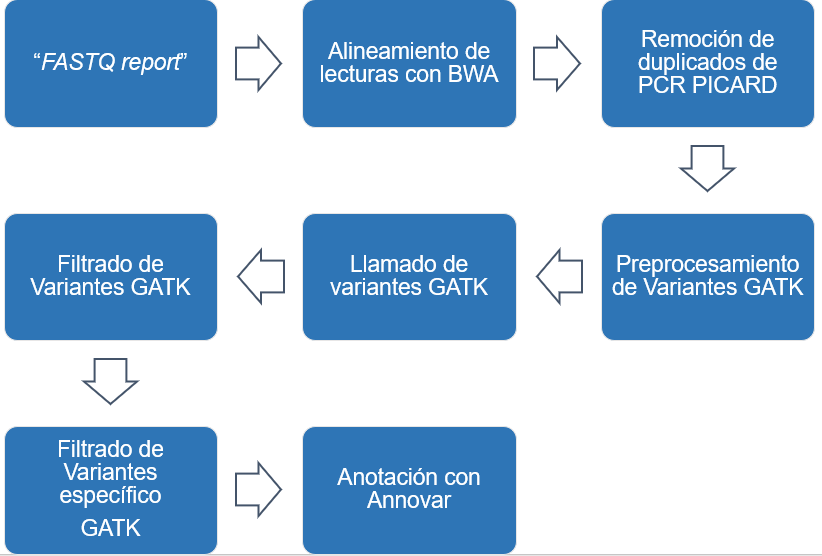
\includegraphics[width=1\textwidth]{pipeline1}
		
	\end{figure}
	
\end{frame}
\subsection{Identificación de variantes}

\begin{frame}{Calidad de la secuenciación}
	\begin{figure}
			\centering
		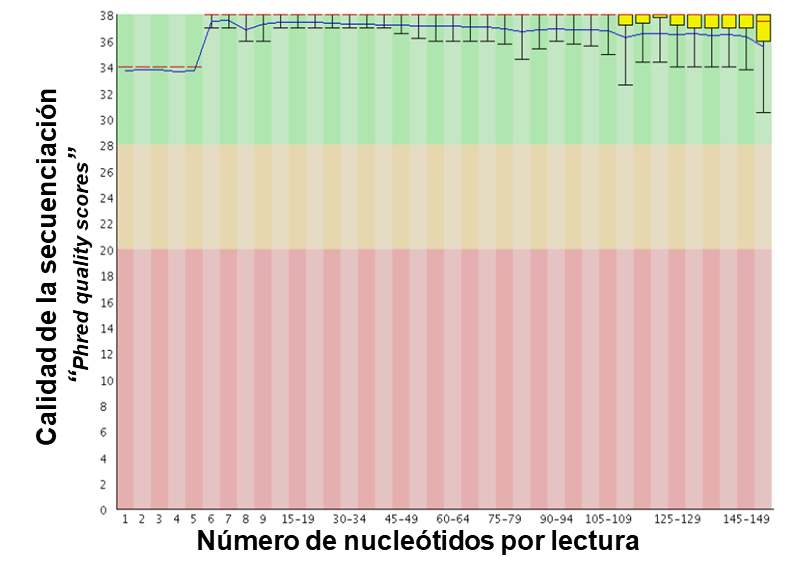
\includegraphics[width=0.8\linewidth]{calidadfastq.png}
		\end{figure}
	\end{frame}

\begin{frame}{Validación}
	
	\begin{enumerate}[1.]
		\item Validación con datos internos. Datos de un paciente con 4813 genes(Illumina).
		\item Validación con datos públicos. Datos del exoma completo NA12878.
	\end{enumerate}
	\centering
	
\includegraphics[width=30mm]{validacion.png}
	
\end{frame}

\begin{frame}{Validación interna}
\begin{table}[h!]
	\centering
	\footnotesize
	\begin{table}[]
		\begin{tabular}{l|l|l|l|l|}
			\cline{2-5}
			& \multicolumn{4}{c|}{\textbf{Variantes}} \\ \cline{2-5} 
			& SNV    & Indels  & Desconocida  & Total \\ \hline
			\multicolumn{1}{|l|}{Pipeline}   & 54538  & 8855    & 122          & 63515 \\ \hline
			\multicolumn{1}{|l|}{Calibradas} & 10425  & 828     & 44           & 11297 \\ \hline
			\multicolumn{1}{|l|}{Illumina}   & 9601   & 436     & 28           & 10065 \\ \hline
		\end{tabular}
	\end{table}
	\caption{Resultados de variantes obtenidas}
\end{table}
\end{frame}

\begin{frame}{Distribución de variantes}
	\begin{figure}[]
		\centering
		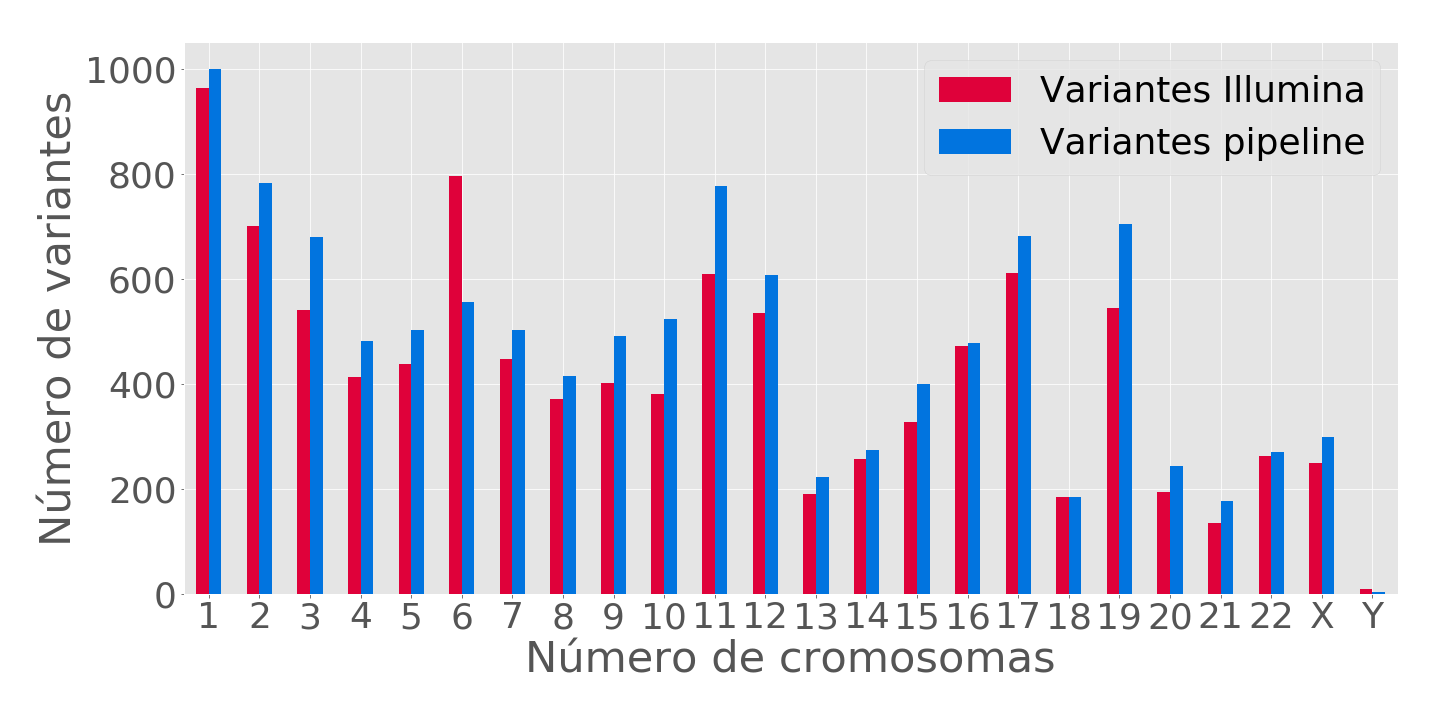
\includegraphics[width=1\textwidth]{validacion1}
		\end{figure}
\end{frame}

\begin{frame}{Validación externa}

Validación con el exoma \textbf{NA12878}
\begin{table}[H]
	\centering  
	\begin{tabular}{l|l|l|l|}
		\cline{2-4}
		& \multicolumn{3}{c|}{\textbf{Variantes Exoma}} \\ \cline{2-4} 
		& SNV           & Indels         & Total        \\ \hline
		\multicolumn{1}{|l|}{Pipeline} & 30893         & 3324           & 34217        \\ \hline
		\multicolumn{1}{|l|}{Públicas} & 29749         & 3101           & 32850        \\ \hline
	\end{tabular}
	\caption{Tabla de Variantes obtenidas a partir de un exoma}
	\label{tabla:tabla2}
\end{table} 
\end{frame}

\begin{frame}{Distribución de variantes exoma NA12878}
\begin{figure}
	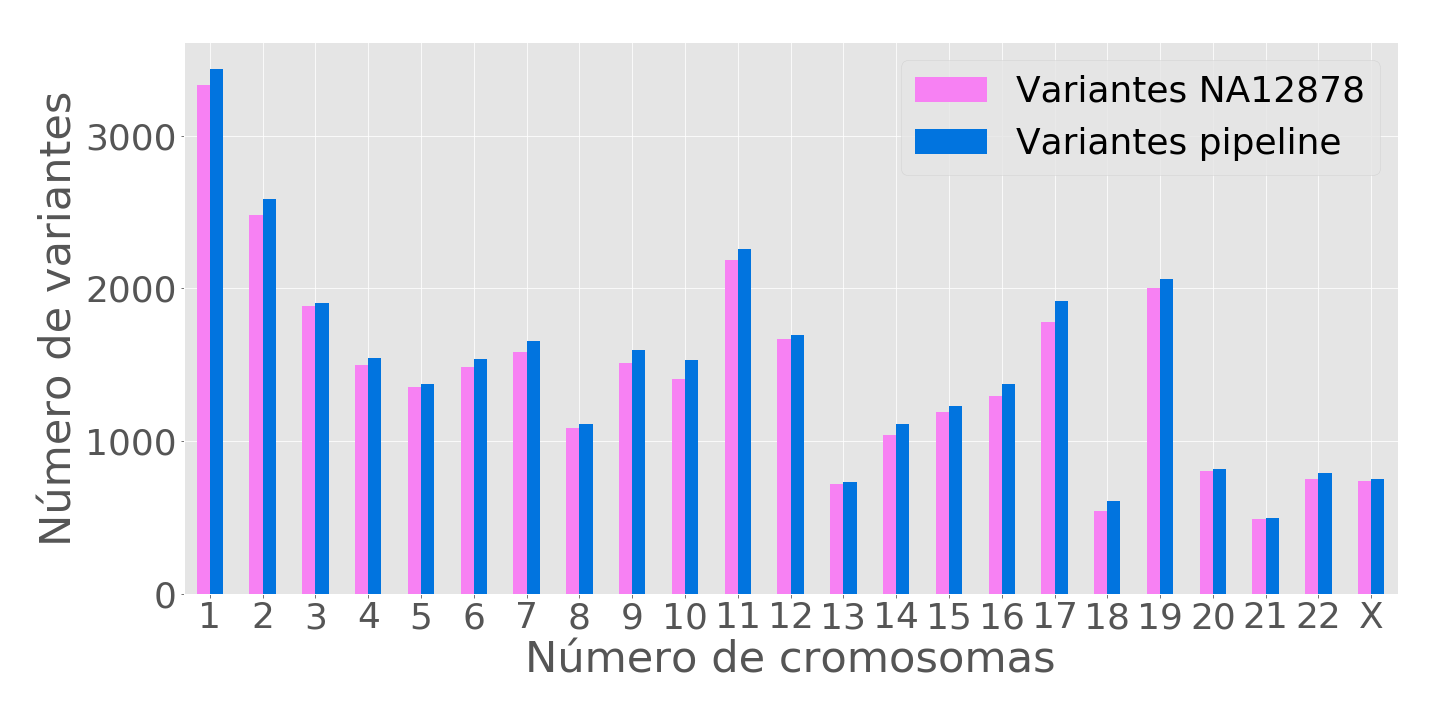
\includegraphics[width=1\textwidth]{validacion2.png}
	\end{figure}
\end{frame}

\begin{frame}{Validación exoma NA12878}
    \begin{table}[H]
	    \begin{center}
		    \begin{tabular}{|l|l|}
			    \hline 
			    \textbf{TP} &  \textbf{TN} \\
			    \hline 
			    32110 & 0  \\ \hline
			    \textbf{FP} &  \textbf{FN} \\
			    \hline
			    1033 &  0\\ \hline
		    \end{tabular}
		\caption{Matriz de confusión}
		\label{tabla:tabla3}
	\end{center}
\end{table}


\begin{table}[H]
	\begin{center}
		\begin{tabular}{|l|l|l|}
			\hline 
			\textbf{Sensibilidad} & \textbf{Especificidad} & \textbf{PPV} \\
			\hline 
			96.88 & 100 & 100 \\ \hline
		\end{tabular}
		\caption{Análisis de sensibilidad y especificidad}
		\label{tabla:tabla4}
	\end{center}
\end{table}

\end{frame}

\begin{frame}{Variante en el Exoma NA12878}
	chr10,96541616,96541616,G,A,exonic,CYP2C19
\begin{figure}[]
	 %\centering
	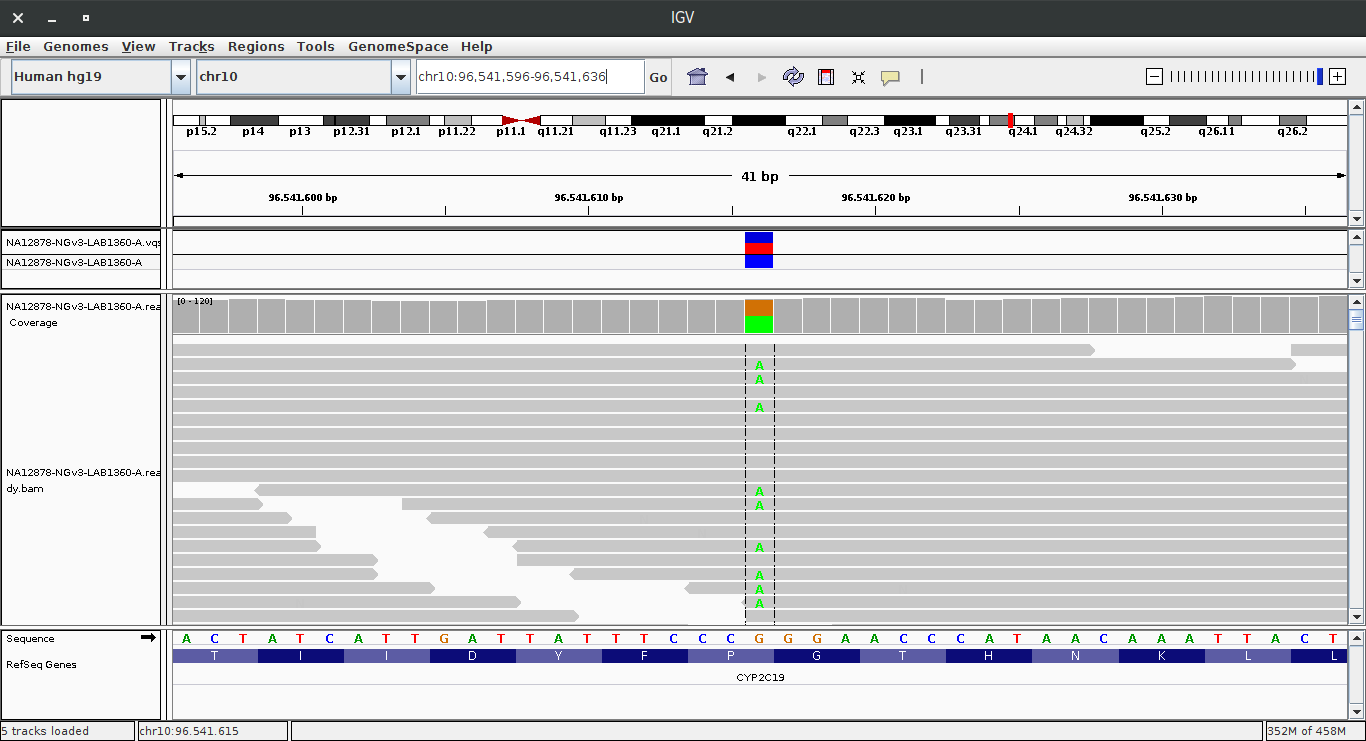
\includegraphics[width=1.02\textwidth]{IGV}
\end{figure}

\end{frame}

\begin{frame}{Historias Clínicas}


\end{frame}

\begin{frame}{Modelo de datos}
Modelo de datos relacional con las siguientes relaciones de información clínica y variantes:
      \begin{figure}
		\centering
		\begin{subfigure}[b]{0.2\textwidth}
			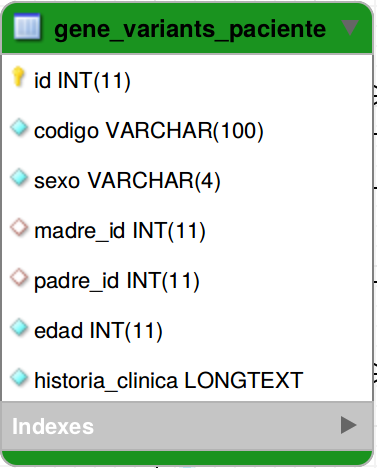
\includegraphics[width=\textwidth]{tabla1.png}
			\caption{Información clínica}
		\end{subfigure}
		\quad
		~ %add desired spacing between images, e. g. ~, \quad, \qquad, \hfill etc. 
		%(or a blank line to force the subfigure onto a new line)
		\begin{subfigure}[b]{0.2\textwidth}
			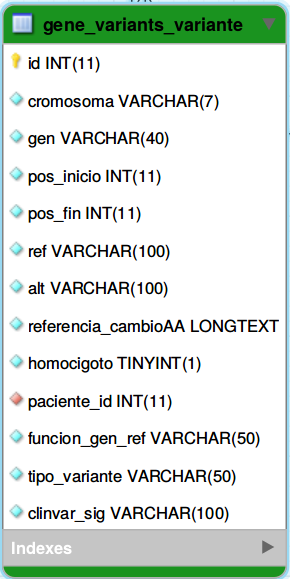
\includegraphics[width=\textwidth]{tabla2.png}
			\caption{Información de variantes}
		\end{subfigure}
	\end{figure}
\end{frame}
    
\begin{frame}{Modelo de datos}
     Relaciones correspondientes a la administración de usuarios y sesiones de la BD:
    \begin{itemize}
    	\item Autenticación de grupos
    	\item Autenticación de usuarios
    	\item Permisos de usuario
    	\item Migraciones de Django 
    	\item Administración de Django
    	\item Sesiones de Django	 	
    \end{itemize}
La Bases de Datos fue implementada en Mysql, y la interfaz en Django.
\end{frame}



\begin{frame}{Interfaz de consulta}
	\begin{figure}
		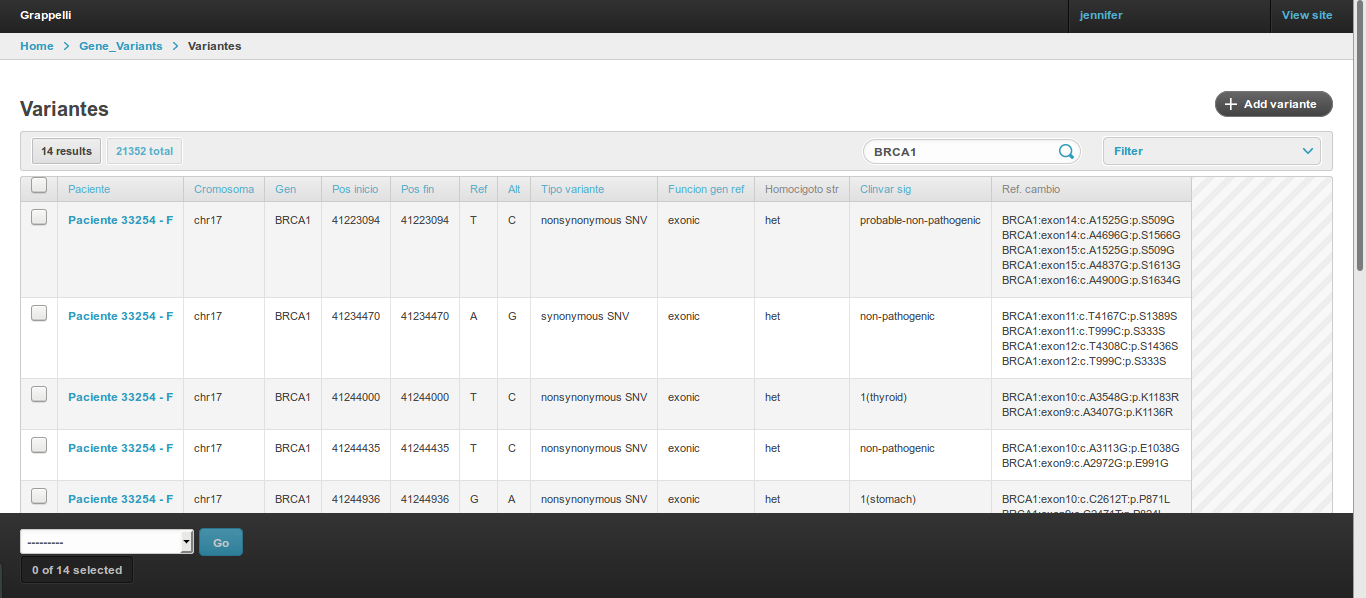
\includegraphics[width=\textwidth]{consulta}
		\newline
		\text{Consulta por Gen}
	\end{figure}
\end{frame}
\section{Minería de datos}
\subsection{Preprocesamento}

\begin{frame}{Modelo propuesto}
\begin{figure}
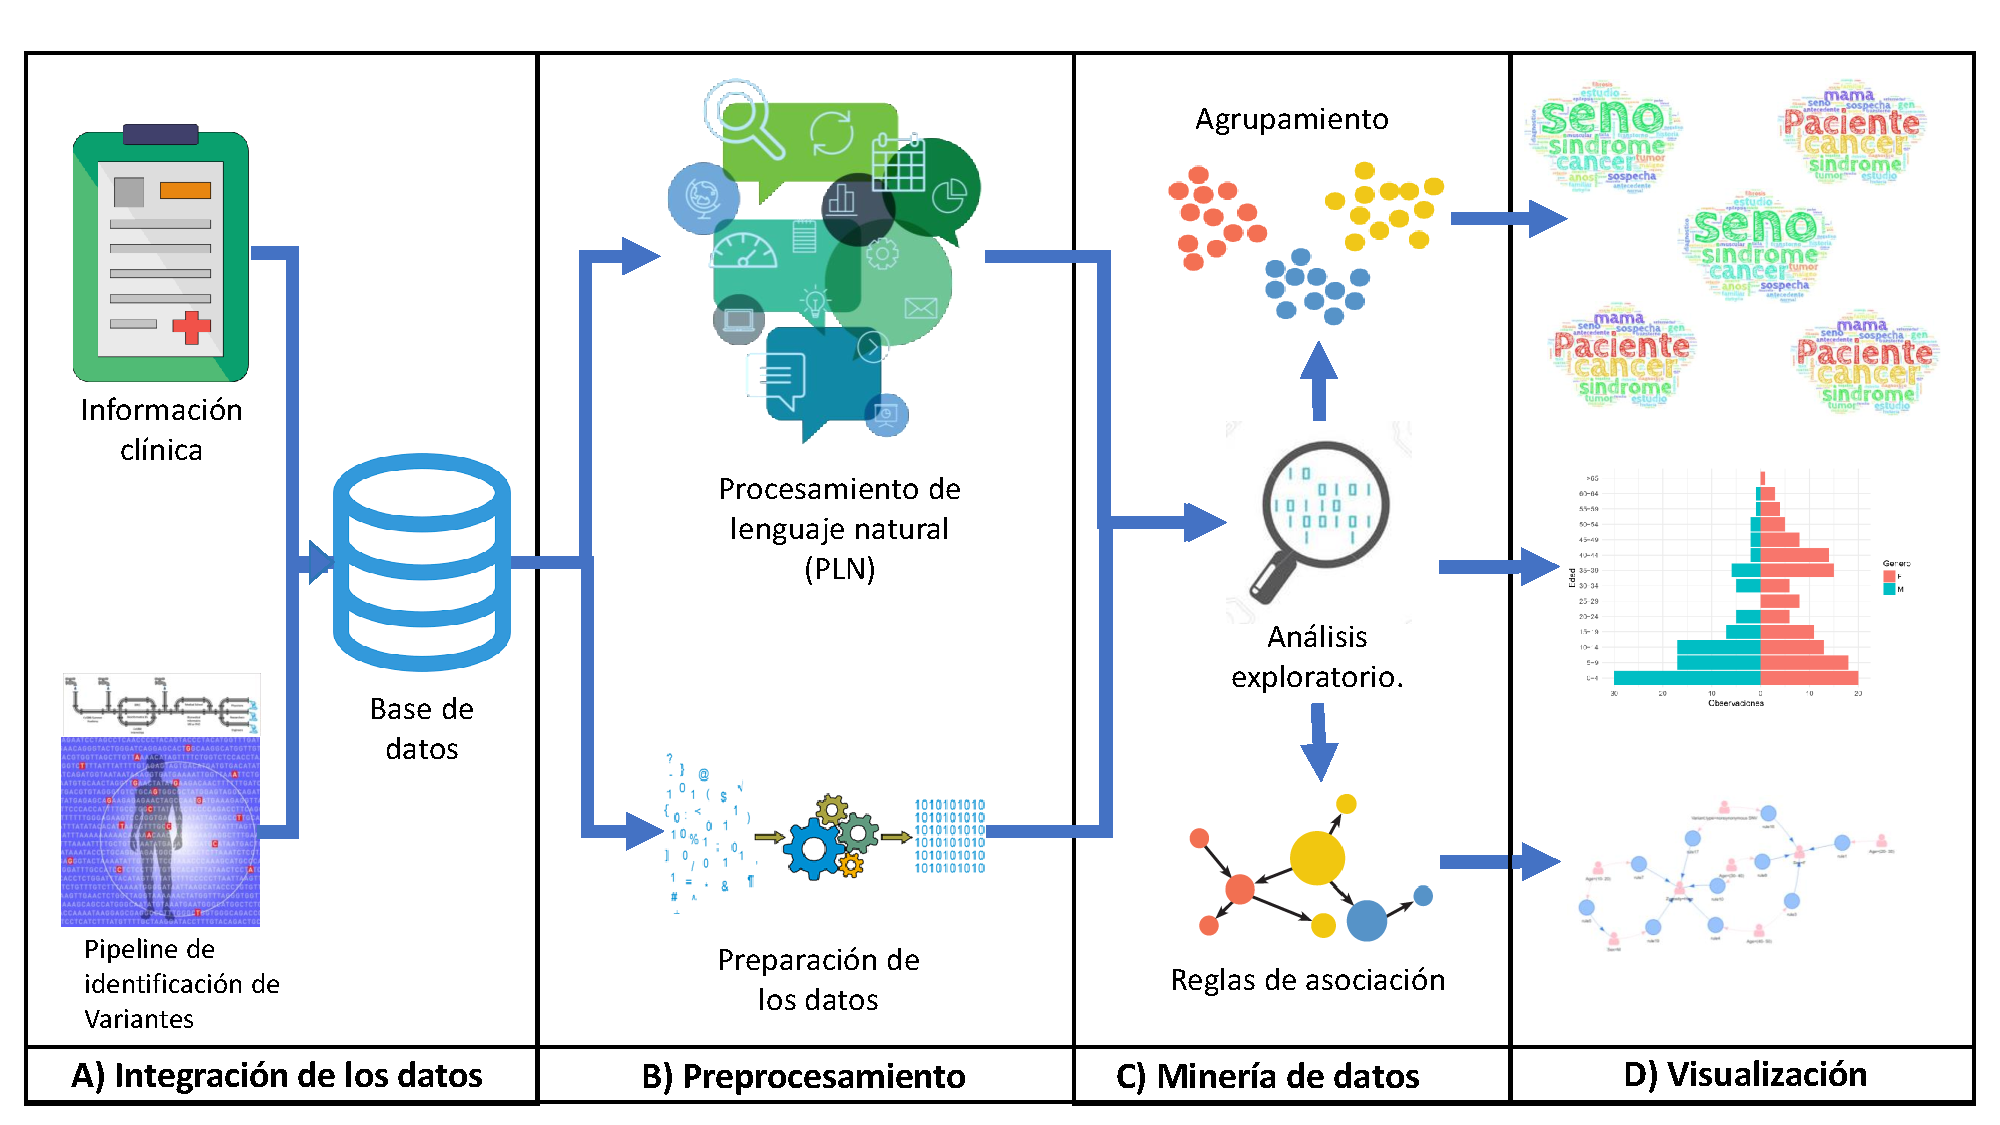
\includegraphics[width=1\textwidth]{KDDtesis.pdf}
\end{figure}
\end{frame}

\begin{frame}{Caracterización de la información clínica}
\begin{block}{}
\justifying
	{\justifying Es necesario caracterizar las historias clínicas de acuerdo al diagnóstico de los pacientes para poder asociar dichos diagnósticos con las variantes identificadas en este trabajo. Siendo el agrupamiento un metodología que permite identificar separar conjuntos de datos de manera no supervisada.
	}
\end{block}
\end{frame}

\begin{frame}{Preprocesamiento de la información clínica}
   	\begin{enumerate}[1.]
   	
		\justifying 
		\item Remoción de \textit{``stop words''} en español, tildes y caracteres especiales como la letra ñ y  unificación en letras minúsculas.
		\item Creación de un diccionario de sinónimos, donde se reemplazaron palabras que hacen referencia a una misma característica, teniendo en cuenta la interpretación clínica.
		\item Cálculo de la frecuencias de palabras dentro de los documentos. 
		\item Remoción de las palabras que no son factor diferenciador de los diagnósticos, como: \textit{pacientes},\textit{pam}, \textit{secuenciación} y \textit{gen}.  
	   	\end{enumerate}

\end{frame}

\begin{frame}{Variantes como transacciones}
\justifying 
A las variantes se agruparon por gen y tipo de variante, rango de edad y genero del paciente.
    \begin{table}[H]
	\centering
	\resizebox{10cm}{!}{
	\begin{tabular}{ll|l|l|l|l|l|l|}
		\cline{3-8}
		&   & \textbf{Items} & Tipo de variante & Cigocidad & Rango de edad & Genero & Grupo \\ \hline
		\multicolumn{1}{|l|}{\multirow{2}{*}{\textbf{Transacciones}}} & 1 & BRCA1          & No sinónima      & Het       & (30-40)       & F      & C1      \\ \cline{2-8} 
		\multicolumn{1}{|l|}{}                                        & 2 & RB1            & Stop gain        & Het       & (0-10)        & F      & C5      \\ \hline
	\end{tabular}
}
\caption{Items y transacciones}
\label{tabla:items}
\end{table}

\end{frame}


\begin{frame}{Modelo propuesto}
\begin{figure}
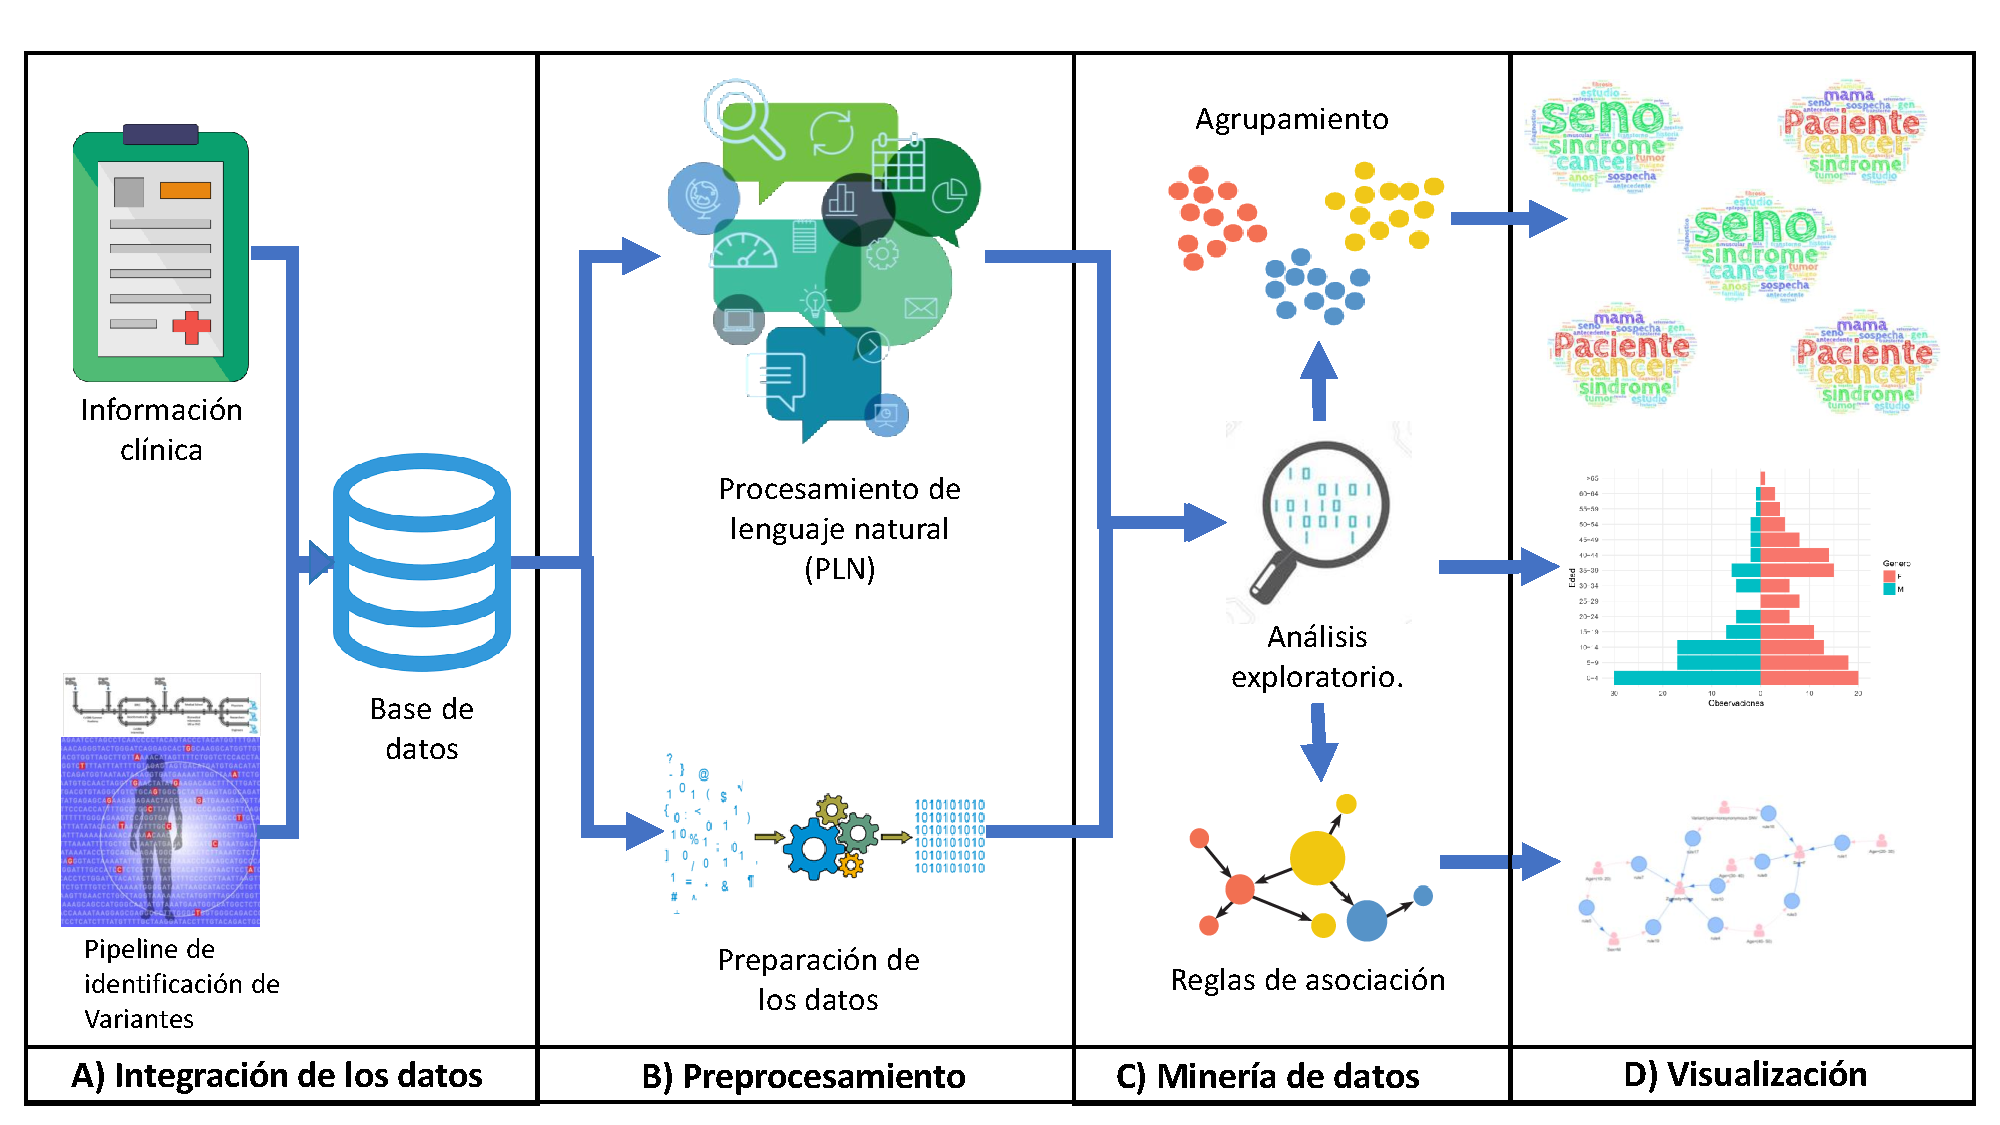
\includegraphics[width=1\textwidth]{KDDtesis.pdf}
\end{figure}
\end{frame}

\begin{frame}{Análisis de términos frecuentes}
	
   \begin{figure}
		\centering
		\begin{subfigure}[b]{0.4\textwidth}
			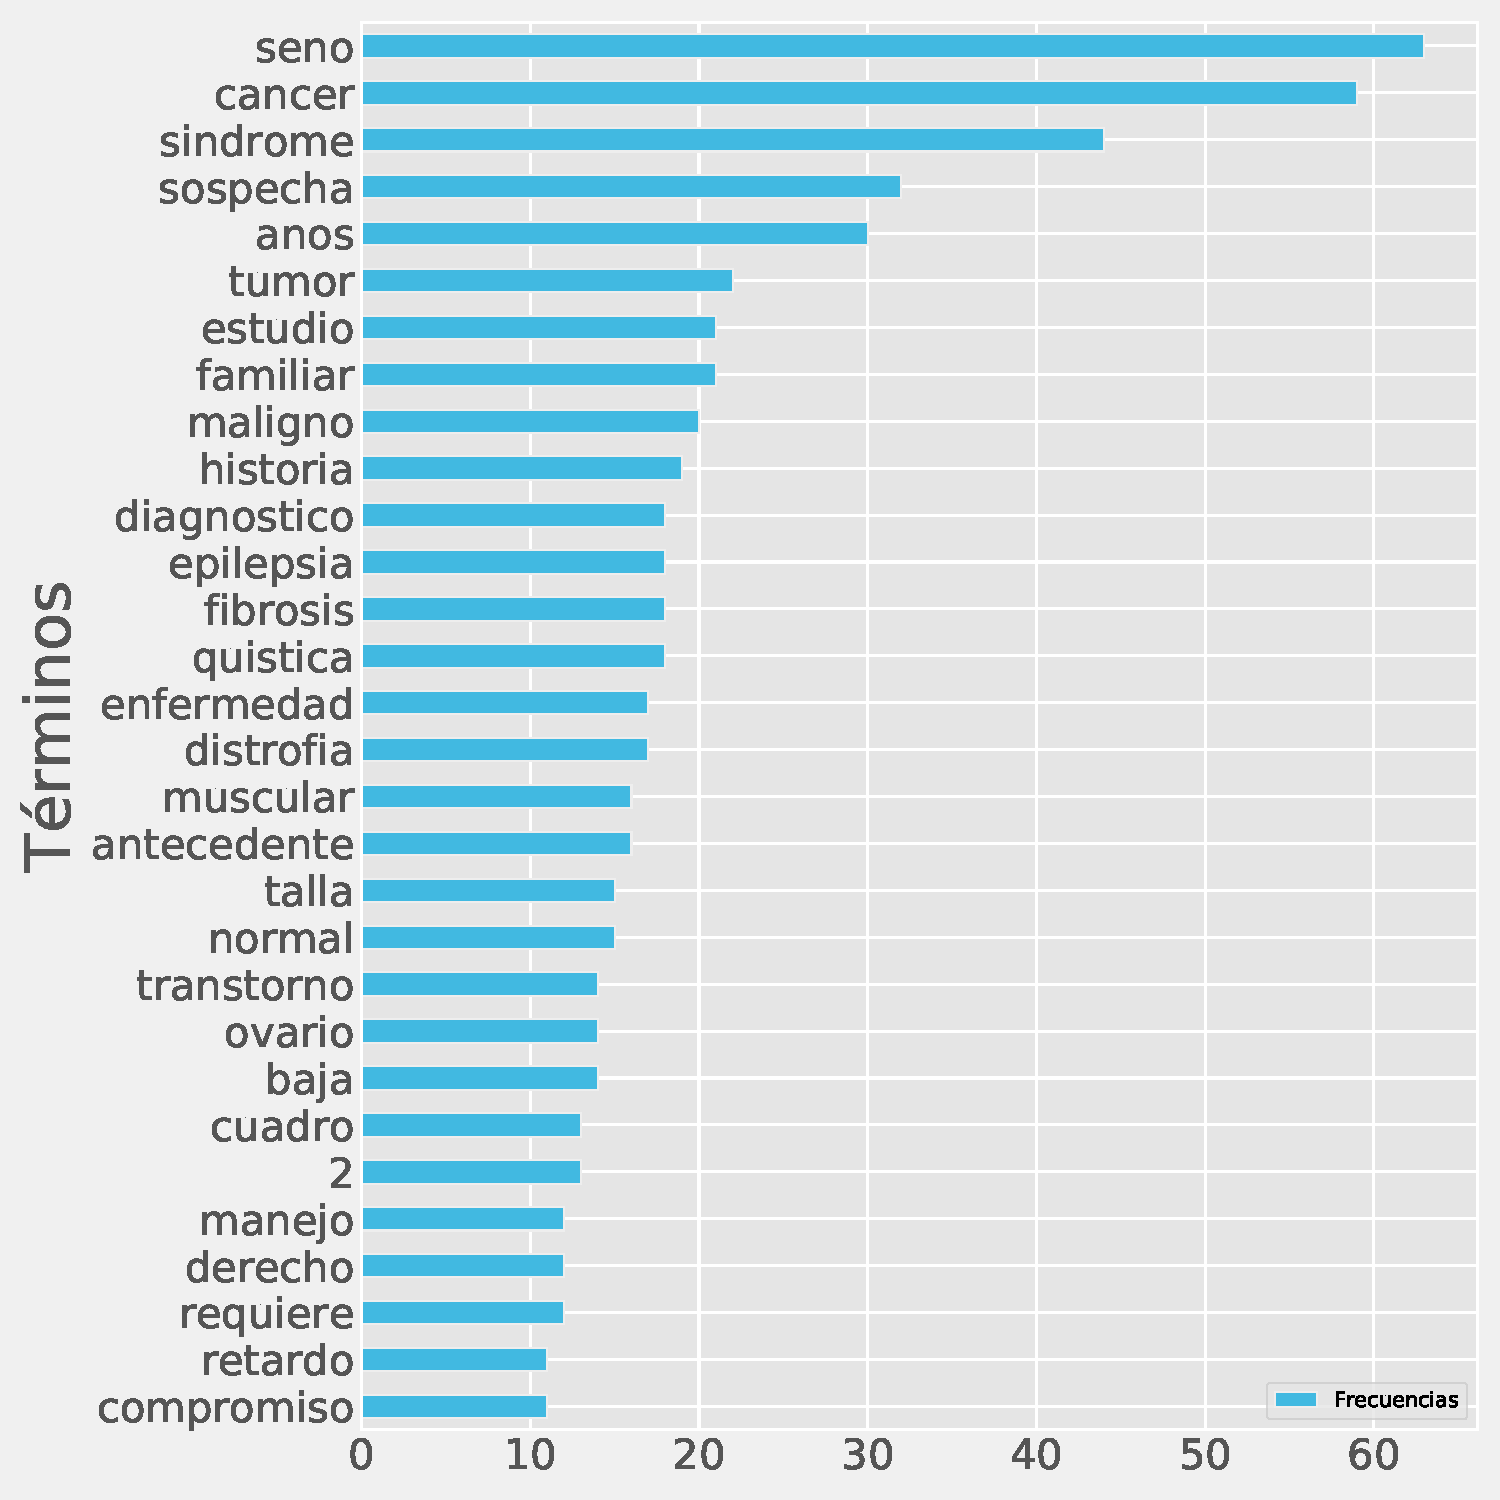
\includegraphics[width=\textwidth]{frecuecias.pdf}
			\caption{Frecuencia de términos}
		\end{subfigure}
		~ %add desired spacing between images, e. g. ~, \quad, \qquad, \hfill etc. 
		%(or a blank line to force the subfigure onto a new line)
		\begin{subfigure}[b]{0.47\textwidth}
			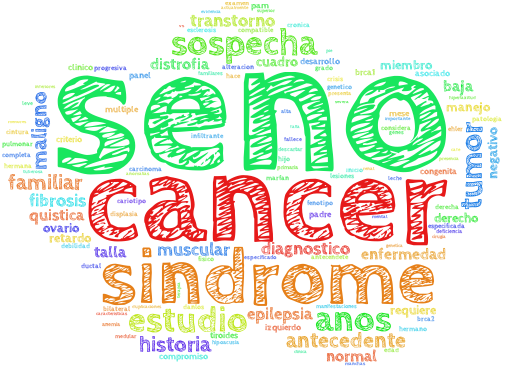
\includegraphics[width=\textwidth]{sin_stop.png}
			\caption{Nube de palabras}
		\end{subfigure}
		%\caption{Representación de términos frecuentes.}
	\end{figure}
\end{frame}

\begin{frame}{Representación tf-idf}
	\begin{equation}
	\begin{gathered}
	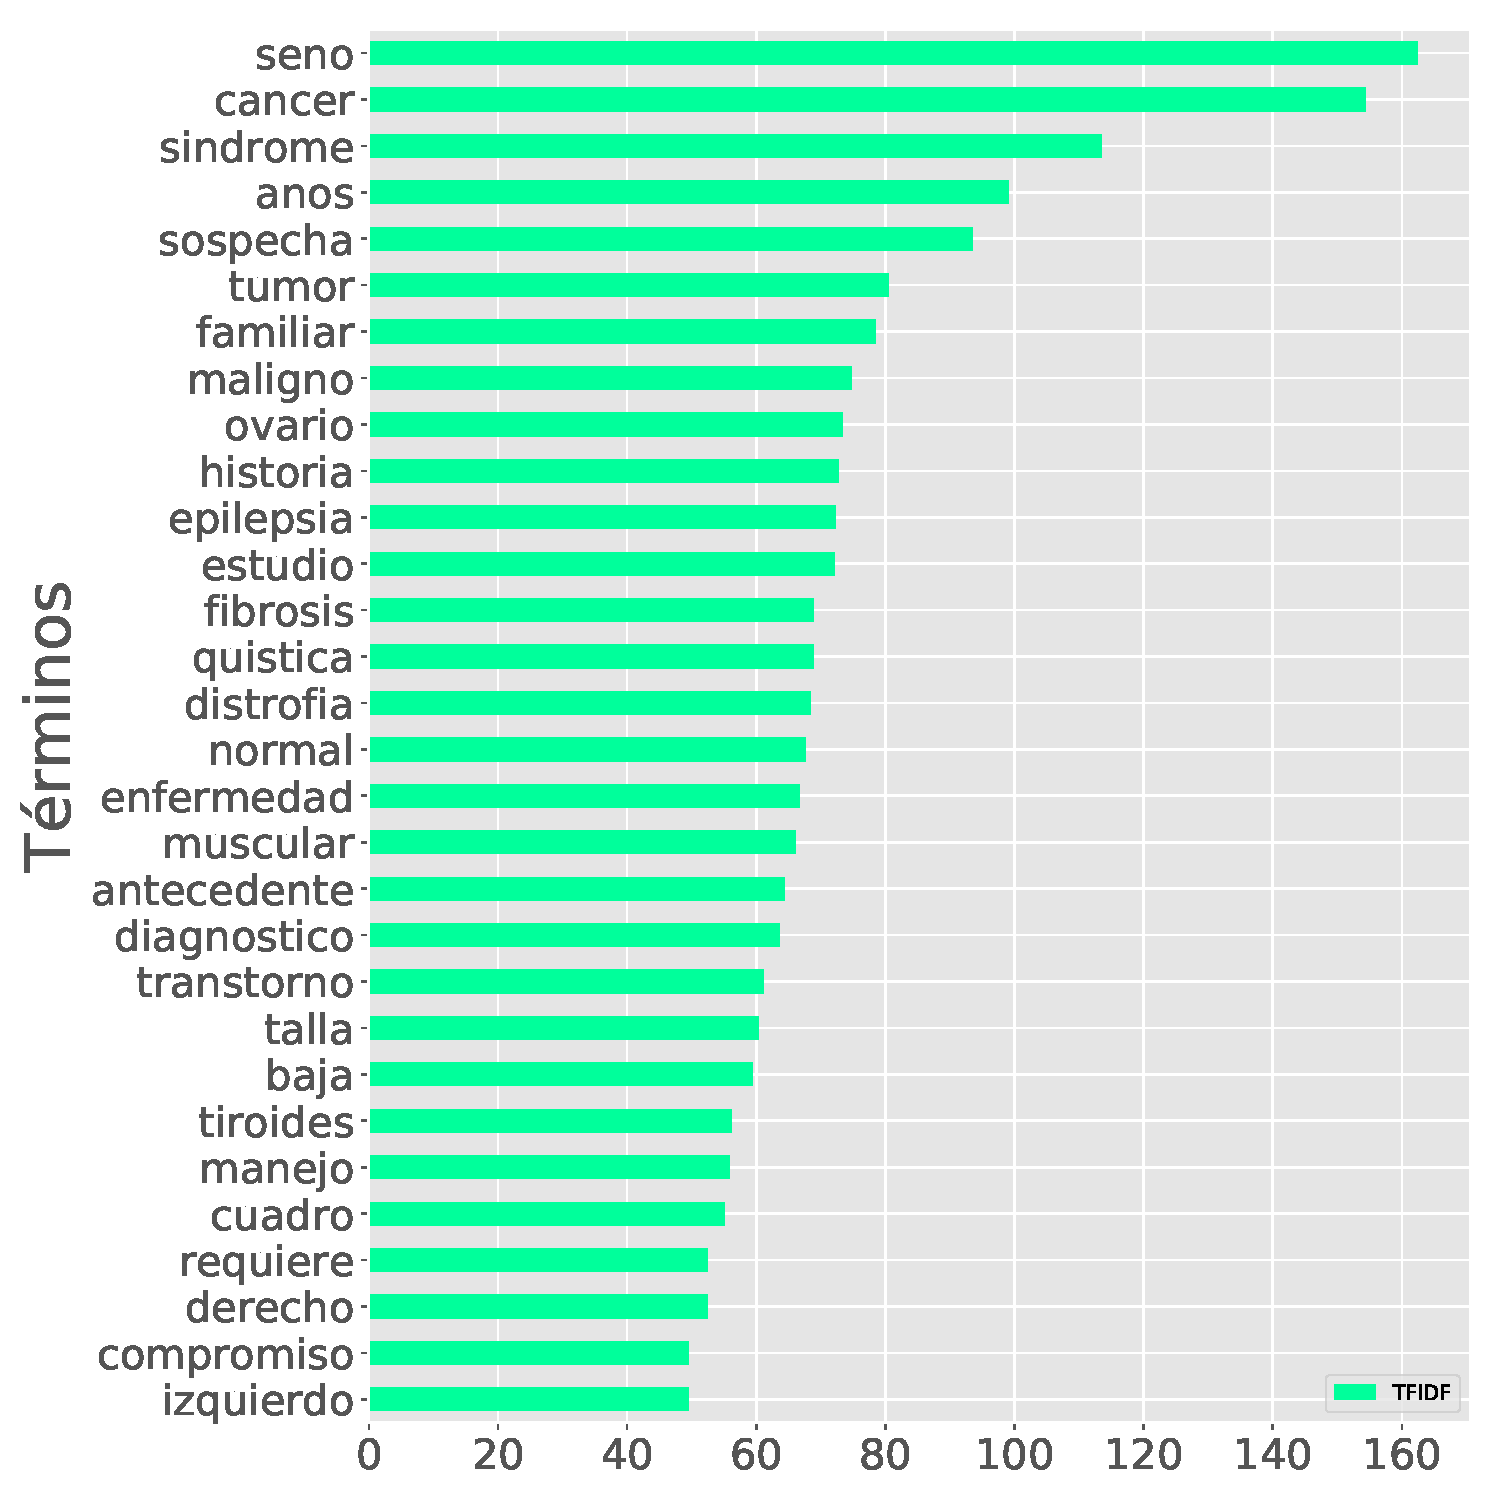
\includegraphics[width=0.5\linewidth]{tfidf.pdf}
	\end{gathered}
	\qquad 
	{tfidf(t,d,D) =  tf(t,d)}\cdot{idf(t,D)}
		\end{equation}
\end{frame}

\subsection{Agrupamiento}

\begin{frame}{Caracterización de la información clínica}
\justifying
Es necesario caracterizar las historias clínicas de acuerdo al diagnóstico de los pacientes para poder asociar dichos diagnósticos con las variantes identificadas en este trabajo. Siendo el agrupamiento un metodología que permite identificar separar
conjuntos de datos de manera no supervisada.

\end{frame}
\begin{frame}{Agrupamiento}
 \begin{figure}
		\centering
		\begin{subfigure}[b]{0.5\textwidth}
			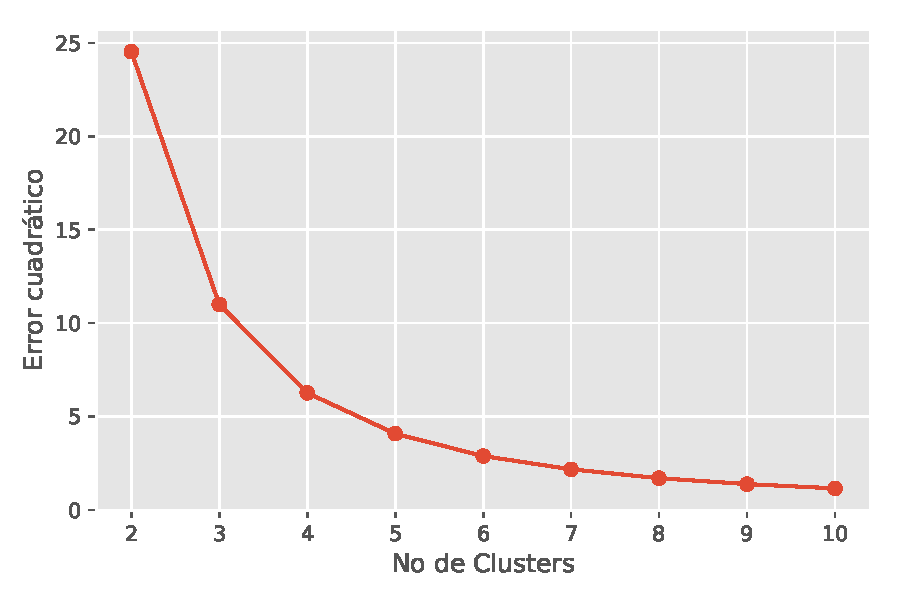
\includegraphics[width=\textwidth]{Clusters.pdf}
			\caption{Error cuadrático}
		\end{subfigure}
		~ %add desired spacing between images, e. g. ~, \quad, \qquad, \hfill etc. 
		%(or a blank line to force the subfigure onto a new line)
		\begin{subfigure}[b]{0.35\textwidth}
			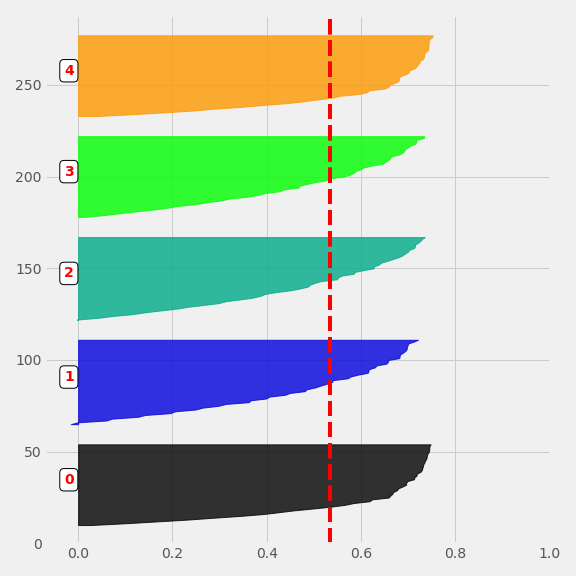
\includegraphics[width=\textwidth]{S.png}
			\caption{ Coeficiente de Silhouette}
		\end{subfigure}
		\caption*{Medidas de selección de número de grupos}
	\end{figure}
\end{frame}

\begin{frame}{Agrupamiento aglomerativo jerárquico usando ``average"}
 \begin{figure}[H]
		\centering
		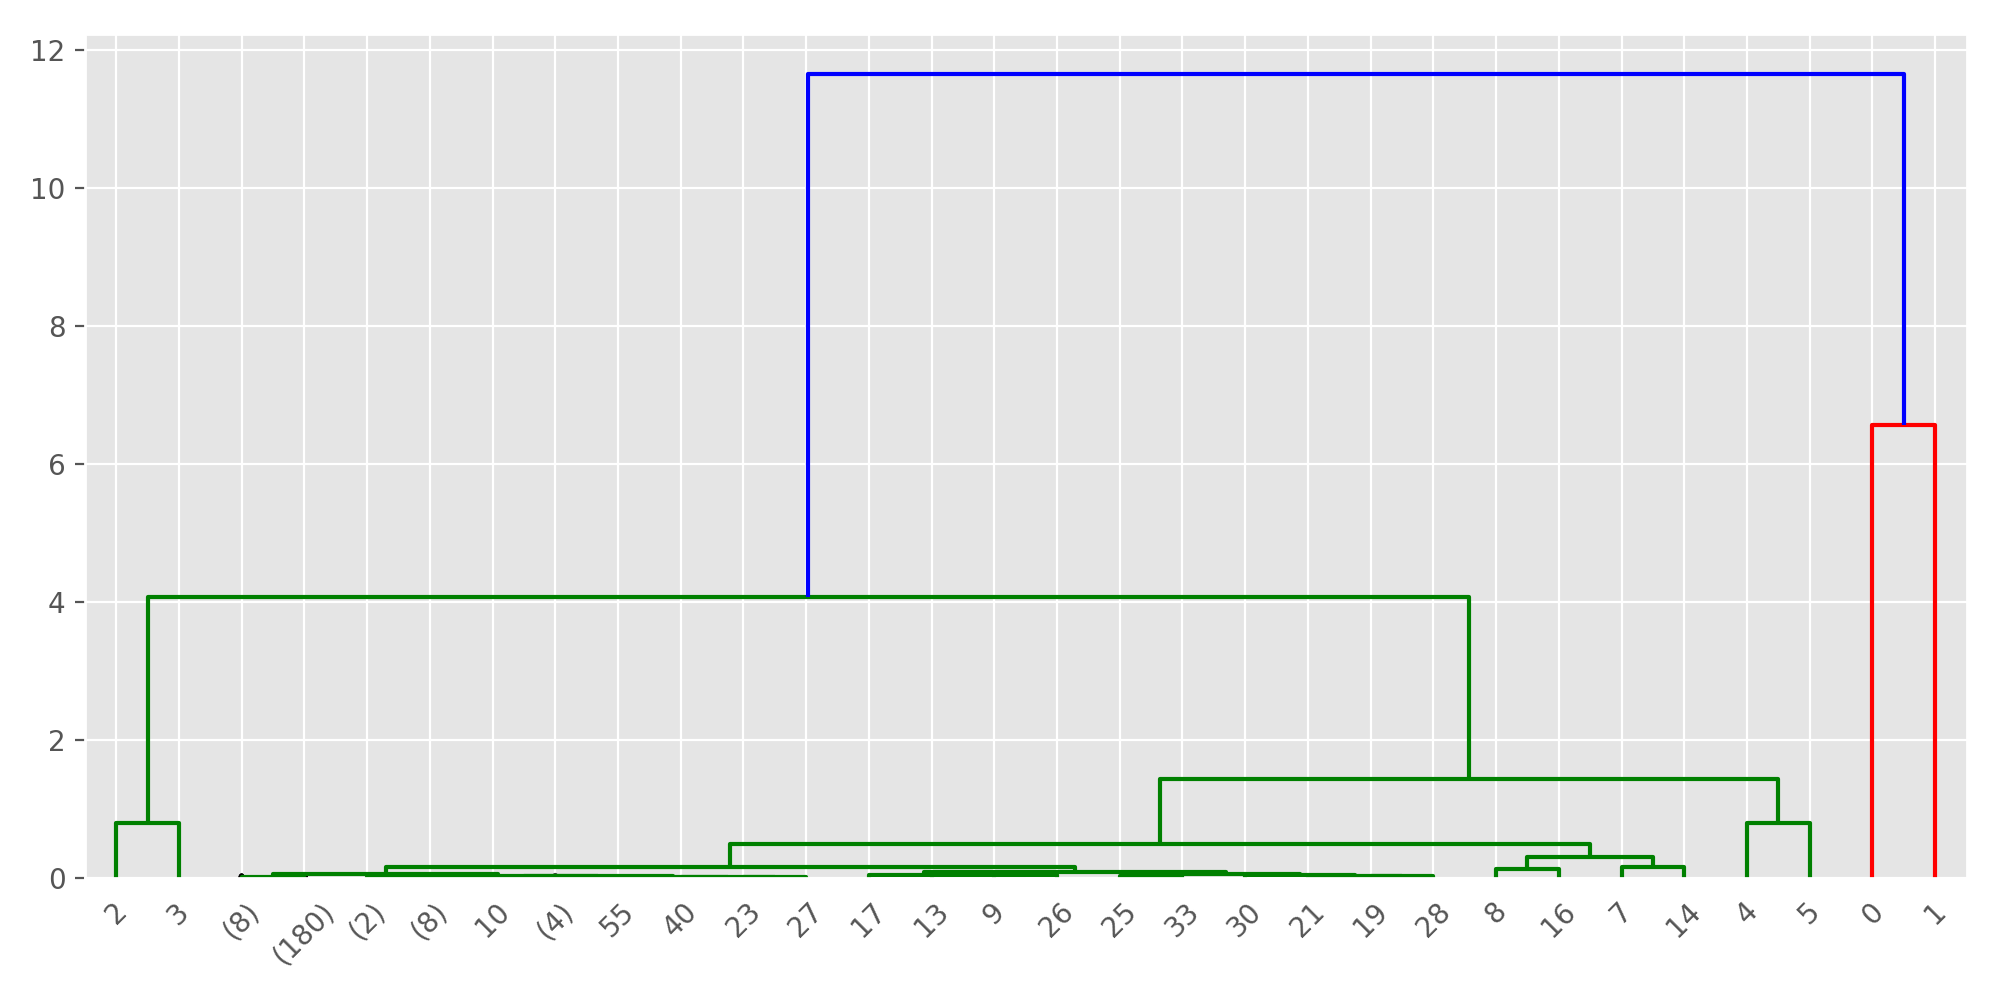
\includegraphics[width=0.9\textwidth]{averagercortado.png}
		\centering
	\end{figure}
\end{frame}

\begin{frame}{Grupos obtenidos usado el kmeans}
\begin{columns}
          \column{0.58\linewidth}
             \centering
             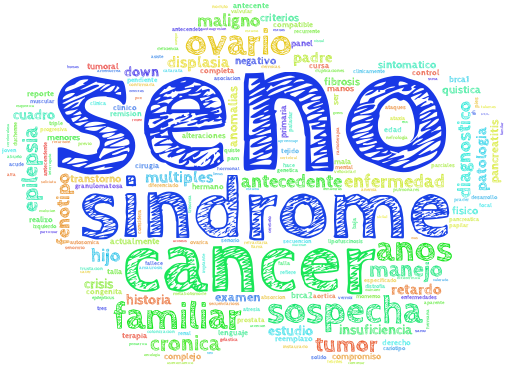
\includegraphics[width=1\textwidth]{cluster1.png}
           \column{0.38\linewidth}
           \justifying
              \textbf{Grupo 1:} Se muestran las palabras más frecuentes que son \textit{seno,sindrome y cáncer}, otras palabras con menor frecuencia son \textit{familiar sospecha y ovario}.
         \end{columns}
\end{frame}

\begin{frame}{Grupos obtenidos usado el kmeans}
\begin{columns}
          \column{0.58\linewidth}
             \centering
             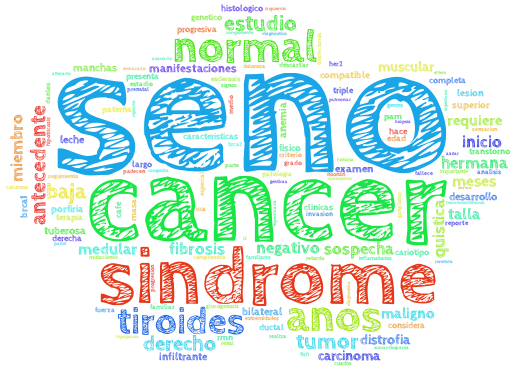
\includegraphics[width=1\textwidth]{cluster2.png}
           \column{0.38\linewidth}
           \justifying
              \textbf{Grupo 2:} Se muestran las palabras más frecuentes que son \textit{seno,sindrome y cáncer}, otras palabras con menor frecuencia son \textit{tiroides anos y normal}.
         \end{columns}
\end{frame}

\begin{frame}{Grupos obtenidos usado el kmeans}
\begin{columns}
          \column{0.58\linewidth}
             \centering
             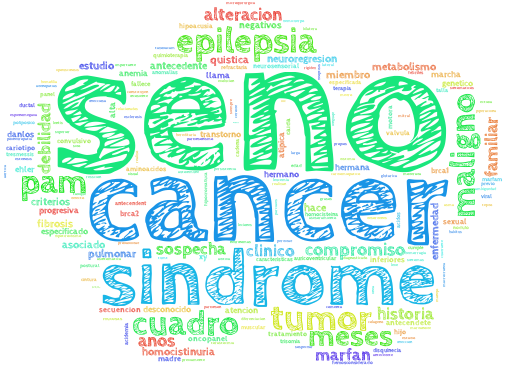
\includegraphics[width=1\textwidth]{cluster3.png}
           \column{0.38\linewidth}
           \justifying
              \textbf{Grupo 2:} Se muestran las palabras más frecuentes que son \textit{seno,sindrome y cáncer}, otras palabras con menor frecuencia son \textit{tiroides anos y normal}.
         \end{columns}
\end{frame}

\begin{frame}{Grupos obtenidos usado el kmeans}
\begin{columns}
          \column{0.58\linewidth}
             \centering
             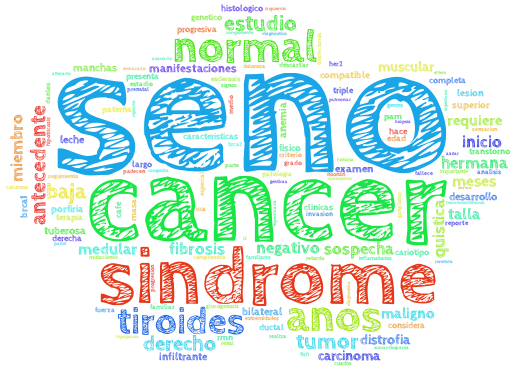
\includegraphics[width=1\textwidth]{cluster2.png}
           \column{0.38\linewidth}
           \justifying
              \textbf{Grupo 2:} Se muestran las palabras más frecuentes que son \textit{seno,sindrome y cáncer}, otras palabras con menor frecuencia son \textit{tiroides anos y normal}.
         \end{columns}
\end{frame}

\begin{frame}{Grupos obtenidos usado el kmeans}
\begin{columns}
          \column{0.58\linewidth}
             \centering
             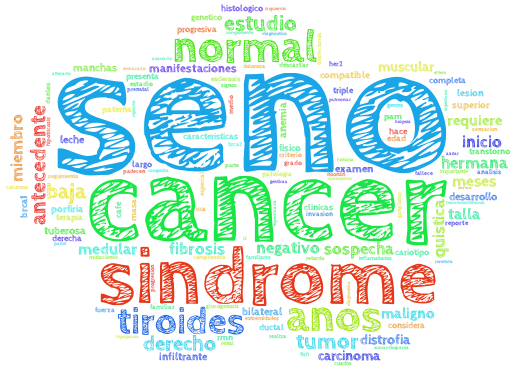
\includegraphics[width=1\textwidth]{cluster2.png}
           \column{0.38\linewidth}
           \justifying
              \textbf{Grupo 2:} Se muestran las palabras más frecuentes que son \textit{seno,sindrome y cáncer}, otras palabras con menor frecuencia son \textit{tiroides anos y normal}.
         \end{columns}
\end{frame}


\subsection{Asociación}
\begin{frame}{Asociación de variantes con grupos de pacientes}
\justifying{
Una vez obtenidos los grupos se utilizó el algoritmo Apriori para obtener reglas de asociación de dos formas: 

\begin{enumerate}
\justifying
	\item Asociación a las variantes por cada grupo de pacientes obtenidos usando el kmeans. 
	\item Asociación a las variantes por toda la información de la base de datos filtrada por los genes CFTR y RB1. 
\end{enumerate}}
\end{frame}



\begin{frame}{Propuesta de visualización de resultados}
Dashboard
\end{frame}

\begin{frame}{Publicaciones}
\begin{itemize}
\justifying
	\item[$*$] Propuesta de pipeline de identificación de variantes. Presentado en el Congreso de Genética Humana.Cali-Colombia 2016.
	\item[$*$] Validación de pipeline para la identifiación de variantes presentado en la Escuela Latinoamericana de Genética Humana y Médica - ELAG. Caxias do Sul, RS, Brasil 2017.
	\item[$*$] Data mining model for the association of genetic and clinical data in Colombian patients.  ISBM, Chicago-USA. 2018 Aceptado. 
	\item[$*$] Association of variants with clinical data in a sample of the Colombian population using the Apriori algorithm. Cabana Travel Fellowships. ISCB-LA SOIBIO EMBnet. Viña del mar-Chile 2018. 
\end{itemize}
\end{frame}

\begin{frame}{Presentaciones}
\begin{itemize}
\justifying
    \item[$*$] Exomic and clinical data management using Django en IV Congreso Colombiano de Bioinformática y Biología Computacional y la VIII Conferencia Iberoamericana de Bioinformática. Cali-Colombia 2017.
	\item[$*$] Propuesta del  modelo de minería en datos clínicos. Conferencia Pycon Colombia.Medellín 2018.

\end{itemize}
\end{frame}
\section{Conclusiones}
\begin{frame}{Conclusiones}

    \begin{itemize}
    \justifying
    \item Colombia no cuenta con un estudio de análisis de variantes y asociaciones clínicas a pesar de que la secuenciación esta disponible en el país. Siendo este trabajo pionero en nuestro país.
    
    \item La cantidad de herramientas para identificar variantes y la falta de consensos estándar dificultan la decisión de cuáles son las mejores herramientas y criterios para validar la identificación de variantes.
    
    \item El modelo presentado permite realizar análisis de variantes a nivel de población y no a nivel de individuo como se realiza actualmente. 
    \end{itemize}
  
\end{frame}

\begin{frame}{Conclusiones}
\begin{itemize}
    \justifying
    \item La utilización de técnicas de minería permiten realizar análisis alternativos de como es la distribución de las variantes en una población, no solo mirando el contexto del gen, si no el estado alélico de las variantes, la distribución por genero, rangos de edad y su posible relación con el fenotipo.
    
    \item El gen RB1 presento variantes patogénicas donde los pacientes fueron portadores y afectados, demostrando que el modelo aplicado es lo suficientemente robusto para mirar el comportamiento de una variante dentro de una población.
\end{itemize}    
    
\end{frame}

\begin{frame}{Conclusiones}
\begin{itemize}
    \justifying
    \item La visualización de los resultados de agrupamiento  y reglas de asociación, permite generar nuevas preguntas con respecto a los datos obtenidos, para proponer nuevas validaciones experimentales.
	
	\item Se presentó una de las primeras base de datos con información de variantes en la población colombiana a nivel de regiones codificantes.
\end{itemize}	
\end{frame}

\begin{frame}{Conclusiones}
 
 \begin{itemize}
    \justifying
 \item Los grupos obtenidos a pesar de compartir palabras de diagnóstico frecuentes en común como seno y cáncer entre sí a nivel de caracterización de variantes son distintos.
	\item Los pacientes que tienen un rango de edad de 0 a 10 años son los que más variantes presentan, pero son los pacientes que menos están representado en las reglas de asociación esto se debe a que hay una alta probabilidad de que sus variantes sean de baja frecuencia.
\end{itemize}
\end{frame}
\begin{frame}{Trabajo futuro}
\justifying 
 \begin{itemize}
 \justifying 

	\item Aumentar la información  como variantes de exomas y genomas, e información de regional de los pacientes para evaluar la distribución de las variantes en la población colombiana.

	\item Desarrollar una base de datos NoSQL para integrar la información procedente de diferentes fuentes y que sea permeable a cambios en el tamaño de la información.
	
	\item Calcular las frecuencias de variantes intermedias de modo que sea posible seleccionar items frecuentes, poco frecuentes e intermedios sin necesidad de que se calcule las asociaciones para todos los ítems. 

\end{itemize}
\end{frame}

\begin{frame}{Agradecimientos}
 \justifying 
    A mi familia que me acompaño en todo este proceso, a Sergio Solano y a Julián Cruz que me apoyaron con sus conocimientos, a la profesora Elizabeth León por dirigir este trabajo y a todo el equipo de Genetix SAS quienes donaron los datos utilizados en este trabajo.
\end{frame}


\renewcommand{\addcontentsline}[3]{}% Remove functionality of \addcontentsline
\renewcommand{\section}[2]{}% Remove functionality of \section

\begin{frame}[allowframebreaks]
	\frametitle{Referencias}
	\bibliographystyle{apacite}
		\bibliography{library.bib}
\end{frame}

\begin{frame}{}
  \centering \Large
	{\fontsize{40}{50}\selectfont GRACIAS!}
\end{frame}

\end{document}
